\documentclass[10pt]{report}

\usepackage{amsmath,amscd}
\usepackage{amssymb,array}
\usepackage{amsfonts,latexsym}
\usepackage[mathscr]{euscript}
\usepackage{graphicx,subfig,wrapfig}
\usepackage{times}
\usepackage{psfrag,epsfig}
\usepackage{verbatim}
\usepackage{tabularx}
\usepackage{pdfpages}

\newcommand{\matlab}[1]{\texttt{#1}}
\newcommand{\setname}[1]{\textsl{#1}}
\newcommand{\Ce}{\mathbb{C}}
\newcommand{\Ree}{\mathbb{R}}
\newcommand{\p}{\begin{pmatrix}}
\newcommand{\pp}{\end{pmatrix}}
\newcommand{\bm}{\begin{bmatrix}}
\newcommand{\bb}{\end{bmatrix}}
\newcommand{\eul}[1]{e^{#1}}

\begin{document}

\title{ \vspace{-30mm} Models of the Neuron (580.639)\\Project 1}
\author{Greg Kiar}

\maketitle
\emph{\b{Preface}} \\
The following paper is a step-by-step evaluation of the project criteria as assigned. Numbers are provided and items are answered corresponding to this format in order to simplify the evaluation of the paper. However, effort was made to ensure continuity between questions and sections to provide literary flow. All code used to complete each part is labelled by name and the question it was used for, and contained within an appendix at the end of this document.
\begin{enumerate}
%
% Q 1
%
\item A primary objective which must be met when completing any type of modeling or experimentation is unit consistency. With the conductance being given with units of $\mu S/cm^2$, the units of the other parameters involved in all of the equations used must be set in such a way that they are numerically consistent. One such example of a fitting parameter set for the model, using our conducatnce as a starting point, is shown below. These values were determined by analyzing known equations such as Ohm's Law or the given the MLE equations and ensuring consistency between both sides of each equation tested.
\begin{itemize}
\item Time: milliseconds, $ms$
\item Current: microamps per centimeter squared, $\mu A/cm^2$
\item Potential: volts, $V$
\item Capacitance: nanofarads per centimeter squared, $nF/cm^2$
\item Conductance (given): microsiemens per centimeter squared. $\mu S/cm^2$
\end{itemize}
The solution presented is non-unique to this problem; there are many solutions that could use different units, so long as their magnitudes are balanced in such a way that the equations are satisfied when values are plugged in.
%
% Q 2
%
\item An equilibrium point occurs when all of the differential equations of a system meet at a resting point (value of zero). More plainly, when plotted, an equilibrium point is the intersection of all of the nullclines (trajectory upon which a derivative is zero) in the phase plane. The two methods implemented here to find the equilibrium points in \matlab{MATLAB} were defining the nullclines as analytical functions and finding their crossing, as well as an iterative technique similar to the Newton Method described in the assignment Appendix. \\ The first method, using analytical expression, was solved with the help of the \matlab{fzero} function to find the zero crossing. The input of this function was the difference between the $V$ and $\omega$ nullcline functions. When this input was zero, it meant that the difference between the two functions was zero and there existed an equilibrium point at that pair of $(V, \omega)$ values. The second, iterative, method for zero finding made use of the original differential equation function provided. This method computed values for the derivative based on a starting point which was arbitrarily set. The value for our starting point was then adjusted by our derivative value, and the proces was repeated. This process continued until the value of our differential was sufficiently small to qualitatively state that no change was occuring (here, $0.0001 mV$ potential and $0.00001$ for $\omega$ activation). Since it is statistically impossible for discrete datasets to have a change of zero, these thresholds were necessary so that the process did not iterate forever. Also, it should be noted that the iterative method used here exploits the fact that this system is assumed to not have any stable limit cycles within the region we are looking for an equilibrium point. If such a limit cycle existed, the method would loop around the limit cycle indefinitely as well and not result in finding an equilibrium point. Later on in this paper, the iterative method was replaced with the Newton iterative method exactly to avoid this assumption - which would often be wrong. \begin{figure}[h!] 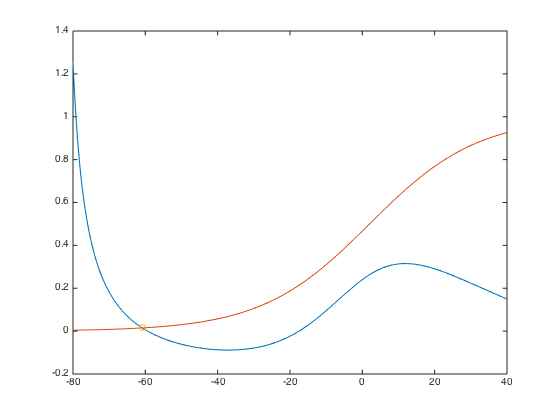
\includegraphics[scale=0.66]{motnq2.png} \caption[h1]{Nullcline trajectories for the MLE system} \end{figure}
%
% Q 3
%
\item Using the methods described in part 2, above, the equilibrium point was found to be at the same location as expected. The equilibrium point for this system was found to be at $(V, \omega) = (-60.8554, 0.0149)$ using my \matlab{fzero} method, and at $(V, \omega) = (-60.8580, 0.0149)$ for the iterative method. The eigen values at the equilibrium point were necessary to compute stability and characterize the equilibrium point. In order to obtain the eigen values, the Jacobian first needed to be computed, and then the eigen values were found by evaluating the determinant of the Jacobian at the point of interest and setting the result to zero. The eigen values computed at this point using the method stated above were $\lambda_1 = -0.0959, \lambda_2 = -0.0366$. These values are both negative which means that this equilibrium point is stable. If one of the points was positive this would be a saddle node, and if they were both positive it would be an unstable equilibrium point. To evaluate consistency of our Jacobian calculation, three methods were tested. The values determined by the \matlab{mlodejac} (provided) and \matlab{numjac} (built-in to \matlab{MATLAB}) corresponded up to four decimal places in each matrix element, so the methods were deemed to be equivalent for later processing in this project. As a third solution, the Jacobian was calculated analytically by hand as is shown below.
\begin{align*}
J &= \bm \frac{\partial \dot{V}}{\partial V} & \frac{\partial \dot{V}}{\partial \omega} \\ \frac{\partial \dot{\omega}}{\partial V} & \frac{\partial \dot{\omega}}{\partial \omega} \bb_{(V, \omega)} \\
\end{align*}
Where, \\
\begin{align*}
\dot{V} & = \frac{i_{ext} - g_{Ca}m_{\infty}(V)(V-E_{Ca}) - g_K \omega (V - E_K) - g_{lk} (V- E_{lk}}{C} \\
\frac{\partial \dot{V}}{\partial V} &= \frac{-g_{Ca}m_{\infty}(V) - g_{Ca}(V -E_{Ca})\p \frac{1}{2 V_2 \cosh(\frac{V_1 + V}{V_2})^2}\pp - g_K \omega - g_{lk}}{C} \\
\frac{\partial \dot{V}}{\partial \omega} &= \frac{-g_K (V - E_K)}{C} \\ \\
\dot{\omega} &= \frac{\phi \p \omega_{\infty }(V) - \omega \pp}{\tau_{\omega }(V)} \\
\frac{\partial \dot{\omega}}{\partial V}  &= \frac{\phi}{2 V_4 \cosh(\frac{V-V_3}{V_4})^2 \tau_{\omega}(V)} + \frac{ \p \omega_{\infty}(V) - \omega \pp \sinh (\frac{V - V_5}{2vV_6})}{2V_6}\\
\frac{\partial \dot{\omega}}{\partial \omega} &= \frac{\phi}{\tau_{\omega}(V)} \\
\end{align*}
After substituting in the values of $(V, \omega)$ at our equilibrium point, the same eigen values were found as using the method above, with the likely addition of rounding error, such that $\lambda_1 = -0.0957, \lambda_2 = -0.0367$. It was also noted that upon opening the function file \matlab{mlodejac} that the expressions matched exactly.\\ Though the section from the R\&E paper was not used as a reference for computing the Jacobian analytically, rather just linear algebra knowledge, the equations were still evaluated to observe where they had made an error. It can be observed from comparing the results obtained here and those published in R\&E that there was a sign error in their equations 7.13 and 7.14. These equations, if used, would dramatically change our evalutation of every system since the equilibrium points would appear to have the opposite stability than they truly did.
%
% Q 4
%
\item In all numerical problem solving, there is a criteria for when the answer produced is sufficiently good. In many cases, such as ours where we seek to find stability, changes between nearby values being approximately zero is the perfect criteria. The tolerance values as stated mean that the system is evaluated until differences between nearby values is less than $10^{-6}$ absolute and $10^{-3}$ relative difference. \\ In our specific case with the use of the MLE equations, the units of electric potential used were $mV$. This scale is appropriate because the range of potential for cells at rest to those at their peak of an action potential is from approximately $-80mV$ to $60mV$, to be generous. Since these equations are being solved for potentials on the same order of magnitude, the tolerance of $RelTol=10^{-3}$ (the smaller of the two tolerances) is equivalent to $1 \mu  V$ of change between nearby values. Because our model, and therefore neurons as this model understands them, are not that sensitive to deviations in electric potential the difference in values once they are on the single $\mu V$ scale are considered completely insignificant. However, if the units used for this systems computation were on the $kV$ scale for some reason, this tolerance would then be in $V$. This would be an issue, because changes observed occur on a $mV$ scale. An equivalent $RelTol$ for the $kV$ instead of the $mV$ scale would be $RelTol=10^{-9}$. Similarly, the principle applies to $AbsTol$ except that the value for $AbsTol$ is multiplied by an extra $10^{-3}$ (as in the \matlab{MATLAB} presets).
%
% Q 5
%
\begin{figure}[h!] 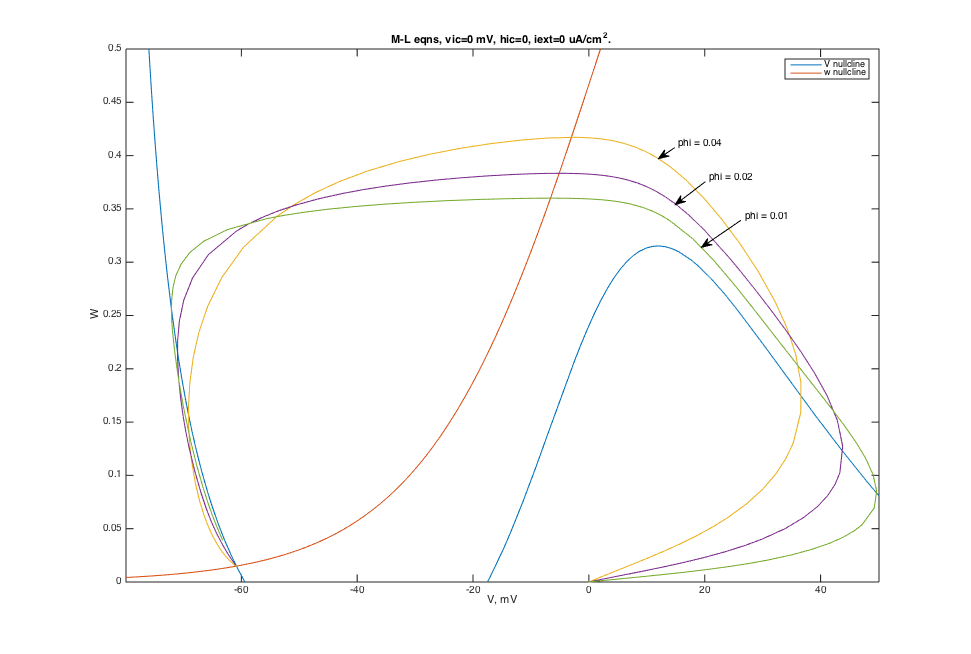
\includegraphics[scale=0.36]{motnq5.png} \caption[h2]{Trajectories affected by varying $\phi$} \end{figure}
\item The phase plane portrayal of a time differential system ignores the time component of the system, and instead plots the change in one parameter dependent on time with respect to the change in another. This is a useful way to observe data so that we can better understand components of our equations and how they affect one another. Here, we test different values for a parameter, $\phi$, on the trajectory of our MLE system in the phase plane. It can be seen from Figure 2, below, that the parameter $\phi$ first of all does not have an effect on the nullclines or equilibrium point(s) of the system. From looking at the MLE equations we can see that the $\phi$ parameter is easily removed when creating the $\omega$ nullcline, and never would have appeared in the $V$ nullcline. This can be confirmed in Figure 2.  Where a change is noted with varying $\phi$ is in the trajectory of the system. It can be seen that with a larger $\phi$, the graph approaches the $\dot{\omega}$ nullcline more quickly than in the cases with a smaller $\phi$. In the extreme case, where $\phi = 0.01$, we see that the trajectory around the nullclines is very heavily dictacted by the $\dot{V}$ nullcline. This is significantly less prominent when $\phi = 0.04$, as the $\dot{\omega}$ function is larger compared to $\dot{V}$ than when $\phi =0.01$. 
%
% Q 6
%
\\
\item In oder to verify that it is equivalent to displace a system by some potential instead of applying current, we must derive a relationship between them. We will first derive a term for the initial voltage, $V(0)$, with no external current applied ($i_{ext} =0$). Calculating $V(0)$ is as follows:
\begin{align*}
V(0) &= \int_{-\infty}^0 \frac{I_{ion}(t)}{C} \mathrm{d}t \\
V(0) &= V_0 \\
\end{align*}
Where $V_0$ is the solution of the above integral. \\
Now, if an external current is added that is non zero and instantaneous at $t=0$, the current could be shown as $i_{ext} = i_0 \delta(t)$. The voltage now also depends on that described above as well as a term in the form of $i_{ext} = \frac{i_0 \delta(t)}{C}$. Solving $V(0)$ now is as follows: \\
\begin{align*}
V(0) &= \int_{-\infty}^0 \frac{I_{ion}}{C} \mathrm{d}t + \int_{-\infty}^0 \frac{i_{ext}}{C} \mathrm{d}t \\
V(0) &= V_0 + \int_{-\infty}^0 \frac{i_0 \delta(t)}{C} \mathrm{d}t \\
\end{align*}
We know that based on the definition of the Dirac Delta function, the following is true:
\begin{align*}
\int_{-\infty}^{\infty} X \delta (t) \mathrm{d}t &= X \\
\end{align*}
Applying this, we find:
\begin{align*}
V(0) &= V_0 + \frac{i_0}{C} \\
V_1 & = V_0 + \frac{i_0}{C} \\
\end{align*}
%
% Q 7
%
\item As was proven above, applying a depolarizing voltage as an initial condition is the same as applying an equivalent external excitatory current to the same neuron. When this depolarization is applied to the resting/equilibrium state of the neuron, the neuron must respond in someway in order to return to the equilibrium state. If this depolarization is significant, then an action potential occurs; otherwise, the system simply returns to the equilibrium value without one. Seen below in Figure 3 are the elicited action potentials for different depolarization values of $V$, as well as the phase-plan portrayal of these same initial conditions(note: colours on the two plots do not correspond). As can be seen from the lowest plot illustrated on the left, time response, plot of $V$, depolarizations do not always elicit any response which involves an increase in potential prior to returning to the equilibrium potential. The rest of the plots illustrated, however, do undergo a positive change before returning to the equilibrium potential. If a "threshold" were to exist in this context, I would choose to define it as limit in depolarizaion at which point the system must undergo a positive change in voltage before returning to the equilibrium value. With that definition of a threshold, we can state that there is a threshold present in the MLE model. That being said, there still exists no \emph{hard} threshold for which a full action potential is elicited, but rather the action potential amplitude changes gradually with depolarization.\\ The values for the depolarization chosen ranged from $V_0 = -20mV$ to $-10mV$. From the lines that are plotted below, using a $\phi =0.04$, the value that appeared to serve as a threshold was a depolarizing potential of $V = -14.8781$. \begin{figure}[h!] 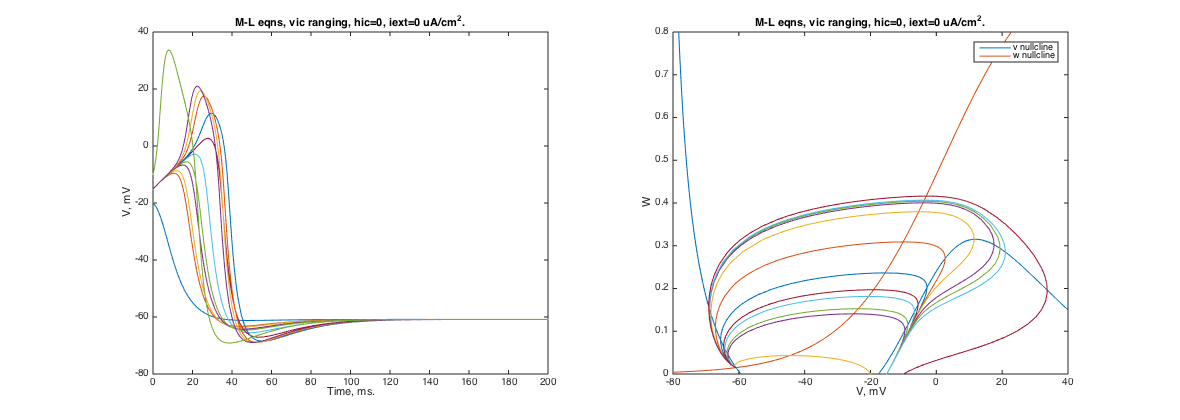
\includegraphics[scale=0.31]{motnq7.png}  \caption[h3]{Demonstration of thresholding in MLE model} \end{figure}
%
% Q 8
%
\item In order to observe the response of our system to different stimulus, and simulate different experiments, several values of initial conditions for a constant applied external current of $i_{ext}=86 \mu A/cm^2$. The initial conditions chosen were the equilibrium potential with the external current at $0 \mu A/cm^2, 86 \mu A/cm^2$, and an arbitrary point which was selected to be $(-27.9, 0.17)$. As seen below in Figure 4, each of the 3 initial conditions showed very distinct responses to one another. The first condition, where the initial condition was at the equilibrium point with $i_{ext} = 0$, we observe a limit cycle around the new equilibrium point. The first several iterations around equilibrium point the trajectory seems to adjust slightly and converge onto a final limit cycle value as is to be expected. The second condition, in which the initial condition is the new equilibrium point, experiences no trajectory in the sense that it is static on the phase plane. This is more valuable than one might expect, since it indicates the stability of the equilibrium point. The third condition spiraled inwards toward the equilibrium point. Consistent with what was observed in the first and third trials, the eigen values at the equilibrium point were $ \lambda_{1,2} = -0.0068 \pm 0.0574i$, which means that we have a stable equilibrium point with spiraling trajectories. \begin{figure}[h!] 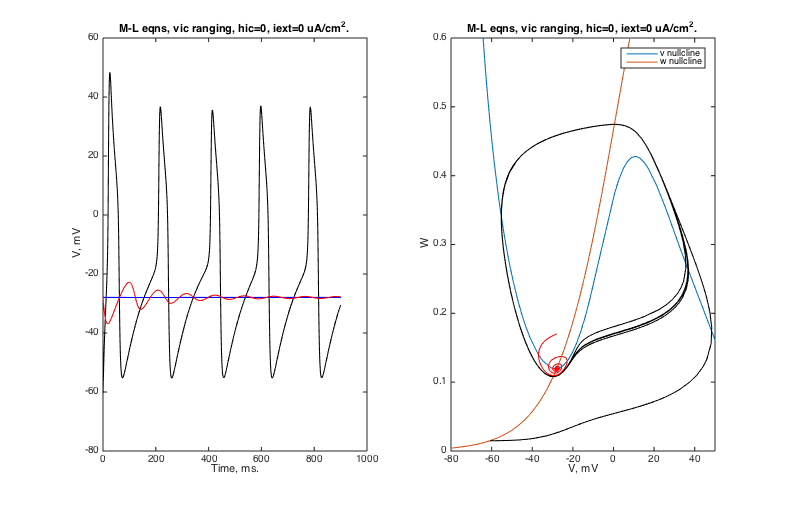
\includegraphics[scale=0.47]{motnq8.png} \caption[h4]{Limit cyles and equilibria} \end{figure}\\ Trials 1 and 2, above are situations which can be useful to impose experimentally. In trial 1, we applied a current offset and sustained it to observe the trajectory of our system when an external current is applied. This is like a current clamp experiment. In the case of trial 2, instead we applied no burst or step of current from the steady state, and simply observe the stability of the equilibrium point. If the system were unstable we would be able to observe an outward spiral of the trajectory from the equilibrium point if any noise existed in the system.
%
% Q 9
%
\item We noticed when applying different sets of initial conditions above, that there exist two stable states in this model when $i_{ext} = 86 \mu A/cm^2$. In order to find the unstable periodic orbit that divides the two stable states, we are able to pull a trick that involves running the system in reverse time. When running in reverse time the differential equations reverse in time. This means that what was a stable point or cycle in positive time, will in fact be unstable in negative time. Knowing this, we are able to evaluate the system in negative time and find exactly the trajectory of the unstable periodic orbit as it exists in positive time. It is important to recognize that the nullclines and equilibrium points do not change when shifting to negative time - this is largely what allows us to complete this substitution. Shown below in Figure 5 is the system running in negative time from two different values: one near the equilibrium point, and one near the outter limit cycle for the positive time case. We can see from this plot that there does indeed exist an unstable periodic orbit separating the two regions in positive time, as here it is a stable orbit. \begin{figure}[h!] 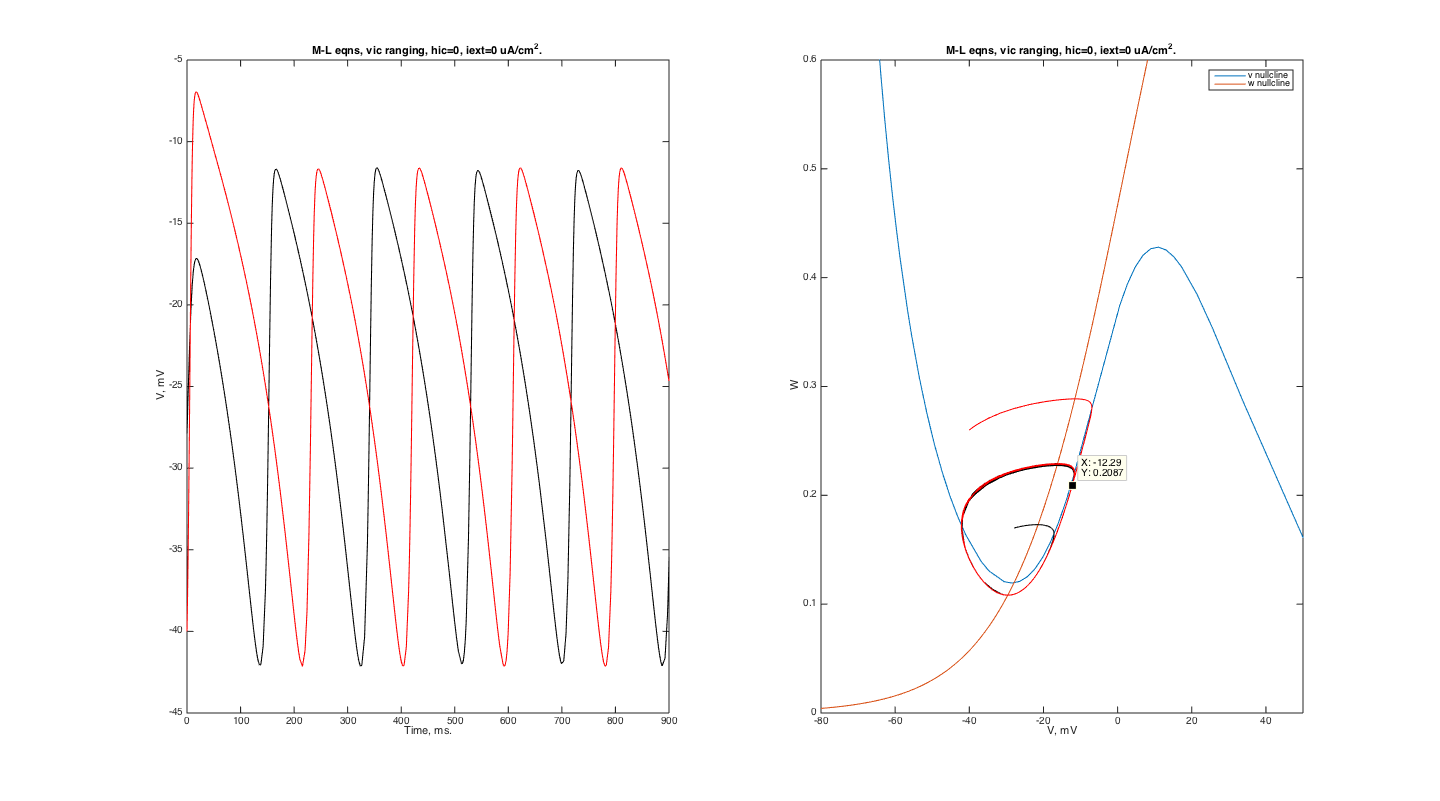
\includegraphics[scale=0.25]{motnq91.png} \caption[h5]{Localization of unstable periodic orbit} \end{figure} \\ In order to obesrve the behaviour immediately around this orbit in positive time, a point on the orbit was selected as a seed and three values were fed into the simulation for positive time. The point directly on the unstable periodic orbit, one slightly inside  of it ($0.01 mV$ left), and one slightly outside of it ($0.01 mV$ right) were the points selected. The resulting trajectories can be seen in Figure 6. We see that the points on either side of the orbit converge to their stable cycle or equilibrium point. We can also see that the point that was started directly on the orbit remains there throughout the duration of the trial. If any noise were added to this system, it would spiral off to one of the two stable states surrounding it. Otherwise, it would continue on this trajectory until stimulus was applied. \begin{figure}[h!] 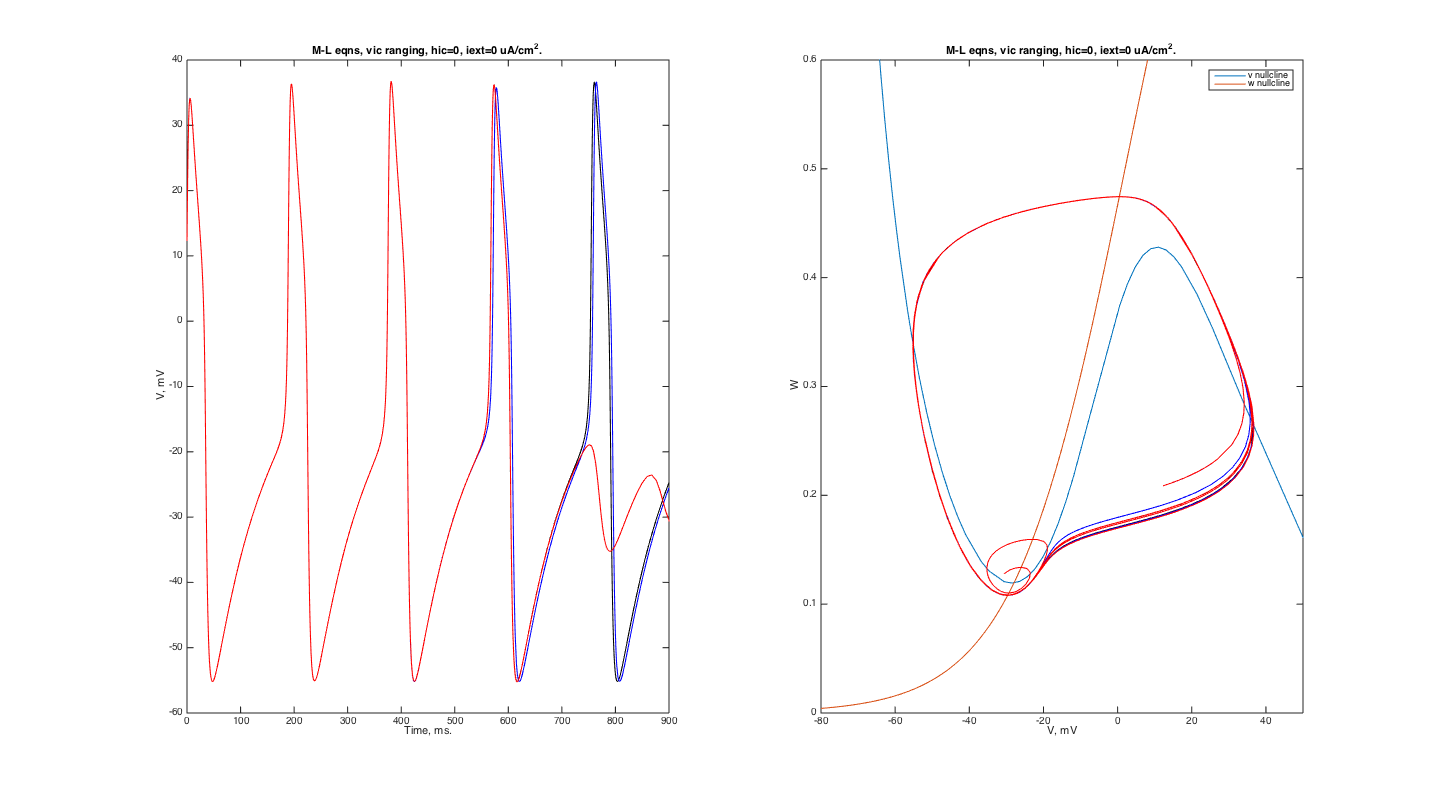
\includegraphics[scale=0.25]{motnq92.png} \caption[h6]{Demonstration of unstable periodic orbit} \end{figure}
%
% Q 10
%
\item A bifurcation is a phenomenon which exists when a sudden change in the characteristics of a system occurs. A Hopf bifurcation, in particular, occurs when the real portion of a pair of complex conjugate eigen values crosses the imaginary axis. From computing and analyzing the eigen values of the system at $i_{ext} = 80, 86,$ and $ 90 \mu A/cm^2$, we can observe that a Hopf bifurcation exists within this region.These eigen values are shown below. \begin{align*} \lambda &= -0.0178 \pm 0.0557i \\ \lambda &= -0.0068 \pm 0.0574i \\ \lambda &=  0.0018 \pm 0.0572i \end{align*} We can tell by observing the eigen values here and seeing that there is a change in sign of the $\Ree$ component of $\lambda_{1,2}$ compared to $\lambda_3$. Since the eigen values at $i_{ext} = 86 \mu A/cm^2$ are negative and complex conjugates of one another, the oscillation corresponds to what we could predict from the eigen values. In order to find a more localized value for where the Hopf bifurcation occures, many currents were analyzed within this reason and Figure 7 was produced. \begin{figure}[h!] 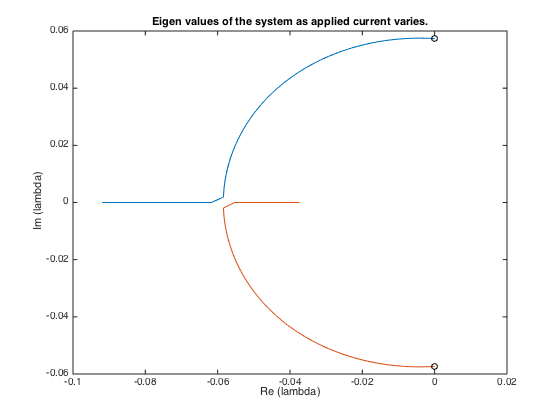
\includegraphics[scale=0.5]{motnq101.png} \caption[h7]{Change in eigen values with varying current towards a bifurcation point} \end{figure} \\ The current which produced the bifurcation (denoted by circles) was $i_{ext} = 89.220 \mu A/cm^2$. When looking at this system near the bifucation point, we observed an oscilation about the equilibrium potential. This observation agrees with our eigen values since they are complex - indicating that they would spiral or oscillate toward their steady state value. To better illustrate the affect of the Hopf bifurcation on the system, Figure 8 shows the rate of firing action potentials for currents ranging below and above the bifucation point. We can see that at the bifurcation current the system behaviour changes dramatically and the firing rate spikes to a non zero value from rest. \begin{figure}[h!] 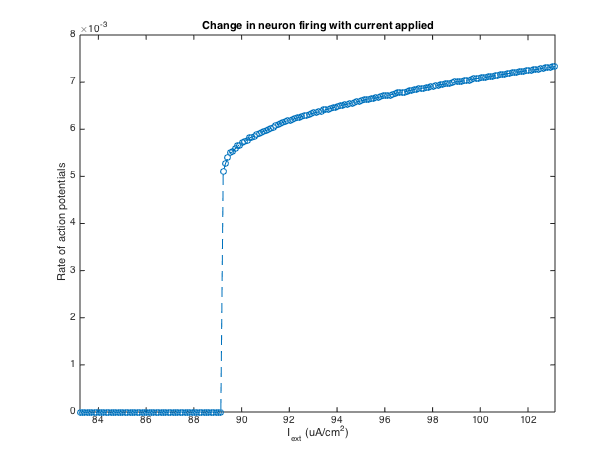
\includegraphics[scale=0.45]{motnq102.png} \caption[h8]{rate of firing with varying applied currents} \end{figure} 
%
% Q 11
%
\item Upon adjusting the parameters in the MLE model to those suggested in the problem statement, we observed three equilibrium points. Characterizing these equilibrium points shows us that, from left to right on Figure 9, they are stable, saddle, and unstable equilibrium points. The equilibrium points for the system described, and plotted in Figure 9, are: \begin{align*} \lambda &= \bm -0.0715 + 0.0000i & -0.1568 + 0.0000i \\ 0.1536 + 0.0000i & -0.0673 + 0.0000i \\ 0.0939 + 0.1723i  & 0.0939 - 0.1723i \bb \end{align*} \\The trajectories plotted in purple and yellow indicate the manifolds of the system. The yellow trajector we notice as the stable trajectory, as it was computed the use of the eigen vector corresponding to the stable component of the saddle point. The purple is the unstable manifold using the same method. What this means, is that the system approaches the saddle node along the stable manifold and attempts to "leave" that region along the unstable manifold. \begin{figure}[h!] 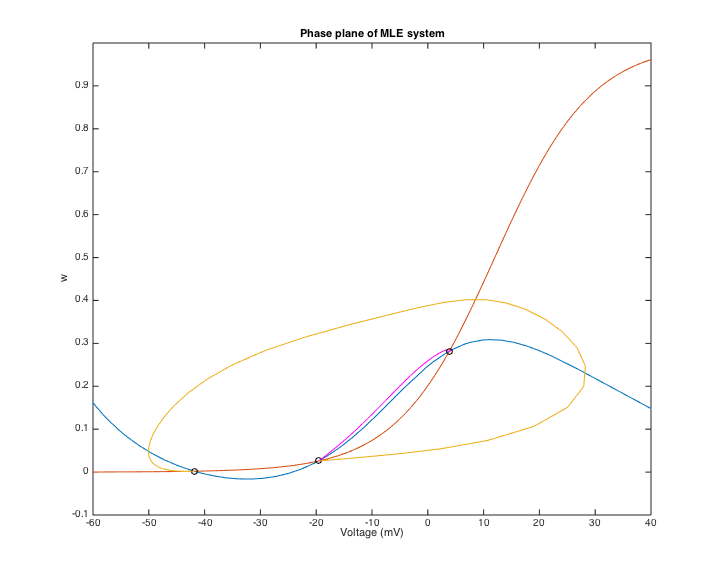
\includegraphics[scale=0.5]{motnq11.png} \caption[h9]{Phase plane demonstration of the system characterized above} \end{figure}
%
% Q 12
%
\item Similarly to what was done for the previous set of parameters in Question 10, here we notice that a bifucation may exist and wish to identify it. The other type of common bifurcation not previously mentioned is a saddle node bifurcation. A saddle node bifurcation occurs when a saddle node and another equilibrium point meet, as the result of shifting nullclines. When these two equilibrium points become one, and then disappear a moment later, the bifurcation occurs. When analyzing this system for $i_{ext}$ between $30$ and $50 \mu A/cm^2$, we noticed that a bifurcation occured at $i_{ext} = 39.6650 \mu A/cm^2$. The characteristic that allows us to observe the saddle node bifurcation is when the determinant of the Jacobian matrix is 0. Since, as was mentioned previously, this is a statistical impossibility with discrete data, we observe this bufurcation by concluding that the determinant of the jacobian is sufficiently close to 0. Exactly at the saddle node bifurcation, two equilibrium points merge by the shift in the nullclines to form one point, immediately before disappearing. This makes sense by observing the determinant to be zero because both components of each set of eigen values should be alike. Shown in Figure 10 is the firing rate of the MLE model at and around this bifurcation point. This saddle node bifurcation appears different from the Hopf bifurtcation in that the firing rate increases much more dramatically in this case as the current increases. \begin{figure}[h!] 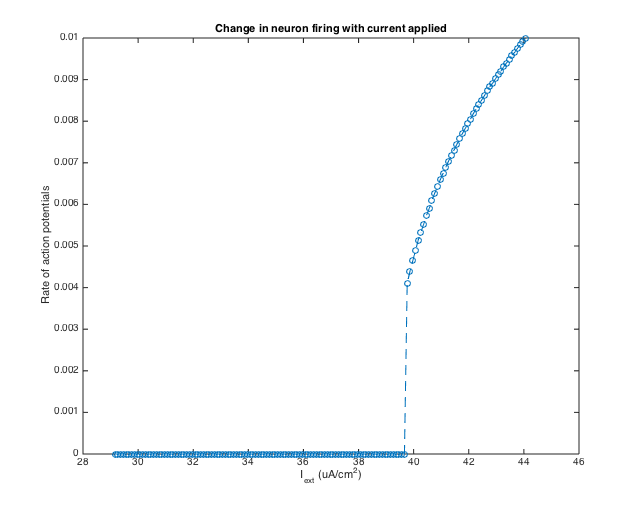
\includegraphics[scale=0.5]{motnq12.png} \caption[h10]{rate of firing action potentials varying with applied currents} \end{figure}
%
% Q 13
%
\item This point in the project indicates a shift in the model being studied. To satisfy this portion, all code pertaining to the HH model of the neuron as can be found in the appendix was created. In order to satisfy a resting potential at $V = -60 mV$, a value for $E_L$ had to be chosen. The value for $E_L$ selected was $E_L = -50 mV$. Plotted in Figure 11 is the Hodgkin Huxley implementation of a neuron basd on this and the given parameters. It can be found from solving this system using Newton method that the equilibrium point occurs at: $ (V, n, m, h) = (-60.153457, 0.315294, 0.051984, 0.601508)$ for this system. The eigen values of this equilibrium point indicate that is a stable equilibrium point.\begin{figure}[h!] 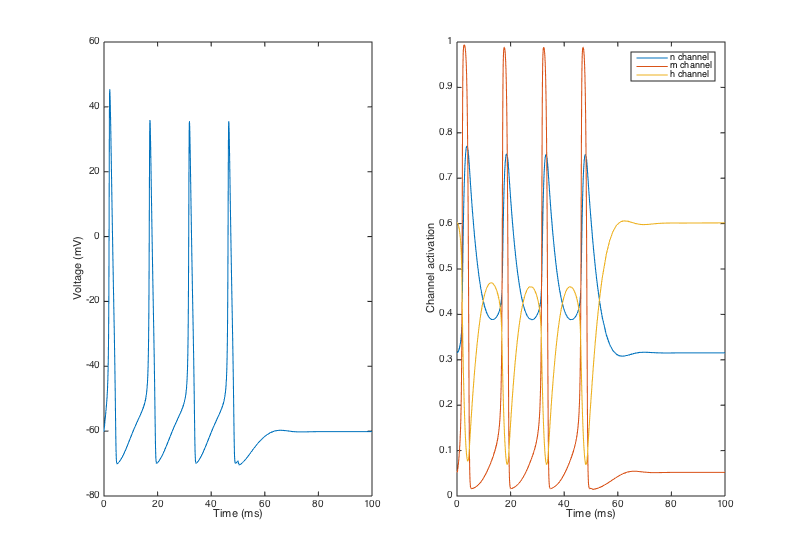
\includegraphics[scale=0.45]{motnq13.png} \caption[h11]{HH model demonstrating several action potentials as it was created using the given parameters} \end{figure}
%
% Q 14
%
\item As was briefly mentioned above, from checking the eigen values at our equilibrium point with $i_{ext} = 0$ it was observed that all of the eigen values were negative, so the system is stable at that point. Since we can represent external currents with depolarizations of the membrane, a depolarizing voltage was applied to observe a threshold for action potentials to occur. When adjusting the depolarization threshold from the euquilibrium point, the deviation required for an action potential to occur was found to be $V_{dep} = 6.61457 mV$. The resulting action potential due to this depolarization is plotted in Figure 12. \begin{figure}[h!] 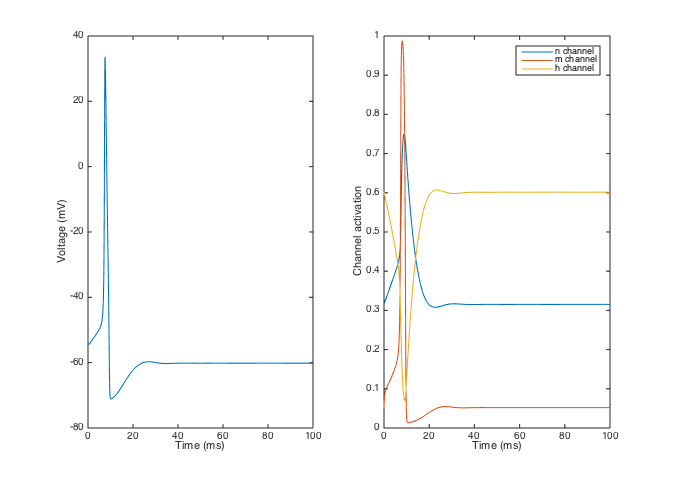
\includegraphics[scale=0.53]{motnq14.png} \caption[h12]{Action potential producted by depolarizing membrane} \end{figure} This plot and depolarization value make sense compared to the Hodgkin Huxley values published in their Fig. 12. The HH figure demonstrates that their smallest depolarization that successfully produced an action potential was $V = 7 mV$. Their figure also shows that a lower potential does not elicit an action potential. In our case, $V = 6 mV$ did not produce an action potential, but a slightly higher value of $V_{dep}$ given above did. Our values agree to the HH values at least within less than a $1 mV$ range from these observations.
%
%Q 15
%
\\
\item In order to analyze bifurcations of this system, it was tested for a range of currents between $i_{ext} = 9 \mu A/cm^2$ and $i_{ext} = 11 \mu A/cm^2$. Knowing that a saddle node bifurcation requires the determinent of the Jacobian to be zero, and a Hopf bifurcation requires the trace of the Jacobian to be zero, both were tested within this range. It was found that a Hopf bifucation occured at $i_{ext} = 9.7882 \mu A / cm^2$. We know that this is a Hopf bifurcation because the real component of the eigen values crossed the 0 boundary, and satisfied the trace criteria. This system is also noted to have bistability. Bistability means that the system posesses more than one stable state. In this case, with one equilibrium point, that means that a stable limit cycle was observed.The phaase plane in Figure 13 shows that at three different starting points, this system either maintained a stable orbit around the equilibrium point or devayed directly into the equilibrium point. Is is important to note that in this phase plane, only the $V$ and $n$ axes are demonstrated, which means that this is not sufficient to do qualitative analysis on but is merely used as an aid for visualization. \begin{figure}[h!] 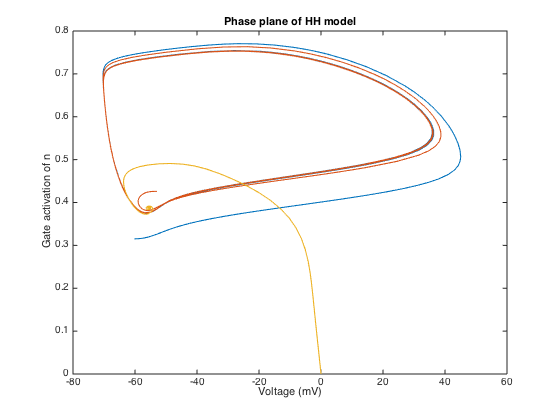
\includegraphics[scale=0.6]{motnq15.png} \caption[h13]{Illustration of the HH phase plane for V and n, showing that there exists both a stable equilibrium point and limit cycle} \end{figure}
%
% Q 16
%
\item Another way to elicit an action potential in neurons, other than depolarizing, is by applying a hyperpolarizing current (at least according to the HH model). This type of action potential is termed the anode-break excitation action potential. In order to obtain this result from our model, we applied a small ($i_{ext} = -3 \mu A/cm^2$) hyperpolarizing current for several $ms$ at the start of our simulation. Figure 14 is the demonstration of this anode break excitation eliciting an action potential. It is observed from the gates, displayed on the right, that the inactivation $h$ gate becomes more open and the two activation $m$ and $n$ gates become less open, or more closed. When the hyperpolarizing current turns off, all of the gates start to reset towards their equilibrium values. During this process, however, we note that the $m$ gate has a significantly faster time constant than either the $h$ or $n$ gates. Because of this rapid opening of the $m$ gates, while the $h$ gates still largely fail to inhibit it, a large spike in ion flux occurs. This ion flux causes the potential of the neuron to rise significantly and initiates an action potential. \begin{figure}[h!] 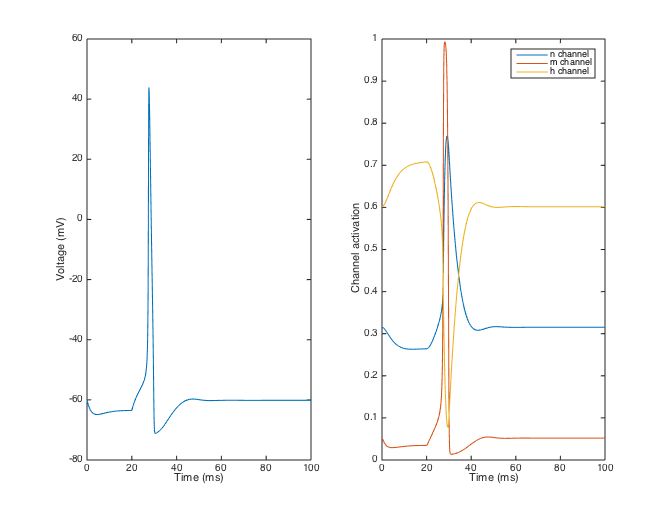
\includegraphics[scale=0.47]{motnq16.png} \caption[h14]{Anode-break excitation spike from the HH model} \end{figure}
%
% Q 17
%
\item As was mentioned above, the anode-break excitation spike is largely due to the behaviour of the $m$ gate responding faster than the inhibiting $h$ gate. In order to simplify our system and observe this on the phase plane, we can set the $n$ and $h$ gate parameters to be constant. We wish to observe the behaviour and location of the equilibrium points of this system for both the steady state, and that underwhich the anode-break spike occurs. The result of this simplification can be seen in Figure 15.  \begin{figure}[h!] 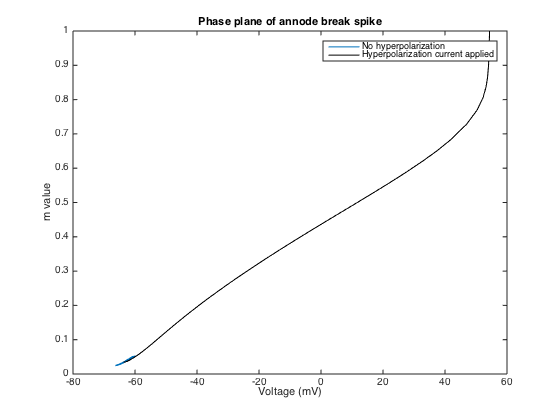
\includegraphics[scale=0.53]{motnq17.png} \caption[h15]{Demonstration of the V, M phase plane during anode-break excitation} \end{figure} \\ The two conditions behave very differently in the phase plane, as could be expected. When the hyperpolarizing current is applied, you can see that the trajectory races toward an equilibrium potential with a large $m$ and positive $V$ value. On the contrary, in the case where there is no hyperpolarizing current, the equilibrium point is nearby the starting condition and the system stabilizes without a spike. As mentioned was observed in Question 16, the $m$ gate rushing to saturation more quickly than the $h$ gate responding to close it is a likely cause for the anode-break spike. The eigen values here for the non-hyperpolarized condition were negative, indicating a stable equilibrium point. For the case of hyperpolarization, the eigen values were positive and complex - which indicates an outward/unstable spiral. When the hyperpolarization disappears, the system will return to the original equilibrium point but will have undergone an action potential in the process.  
%
% Q 18
%
\item In order to understand some more properties about the HH model, it is useful to make an accurate approximation of the model. This is achievable using two things that are known about this system: the $m$ response is much faster than the $n$ and $h$ responses, and the $n$ and $h$ responses occur at a similar rate. Considering the above, we make the approximation that $m = m_{\infty}$. We can also observe the relationship between $h$ and $n$ by plotting them against one another. A nearly linear relationship is observed, so the \matlab{MATLAB} function \matlab{polyfit} was used to find values for the coefficients of the linear relationship. From this, it was found that $h = -1.21n + 0.99$. The value for $m_{\infty}$ was computed based on the $\alpha_m$ and $\beta_m$ coefficients defined in the original ODE solution. The resulting, simplified, ODE system for the HH model is plotted in Figure 16 for an initial condition in which it is stimulated by a short current pulse so that we can observe an action potential for comparison. \begin{figure}[h!] 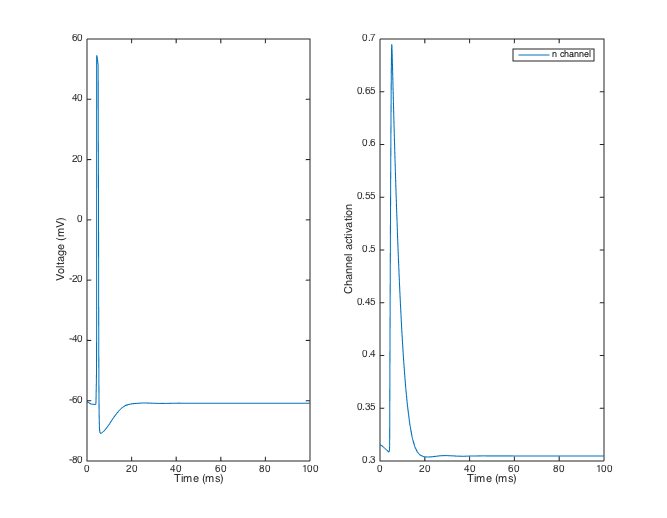
\includegraphics[scale=0.4]{motnq18.png} \caption[h16]{Single action potential demonstrated for the simplified HH model} \end{figure}
%
% Q 19
%
\item In order to feel confident in the simplifications we made to the HH model, we must first compare its output to that of the original HH equations. Through this process we noticed that the approximations made resulted in small changes between the two models but ultimatley the same behaviour is produced. In the observation of an action potential, the simplified model shows essentially fewer "small" changes, such as details in the shape of the refractory period, than the full model. A way I could perhaps more concisely describe this is a low pass filtering of the true response in that the finer detail changes are lost. I think that the reason for the missing small details is simply because we are simplifying them away in the equations through the intense simplification of $h$ and $m$. For instance, $m$ is not immediately $m_{\infty}$, but the approimation is close enough that the general shape of the waveform remains the same. Similarly, this applies to $h$. \\ \\ For the zero current condition ($i_{ext} = 0$) of both systems the equilibrium points for the full and simplified models, respectively, are $(V, n) = (-60.15345, 0.3152)$ and $(-60.8473, 0.3048)$. The equilibrium points also both share the same stability, in that they are both stable and have only real eigen values. When comparing the bifurcation points between the two, we notice that the current to create the bifurcation here is $i_{ext} = 9.7621 \mu A/cm^2$ which is slightly lower than that of the original model though within the range. The voltage offset, $V_{dep}$, required to produce an action potential for the full and simplified models is $V_{dep} = 6.615 mV$ and $6.4210 mV$, respectively. The anode-break behaviour is plotted in Figure 17 for the simplified model. Comparing all of these to the behaviour observed in question 16, we can see that the simplification is quite accurate with respect to the original model. This model, though not statistically proven here, seems to be a valid and userful simplification from the standard HH equations. \begin{figure}[h!] 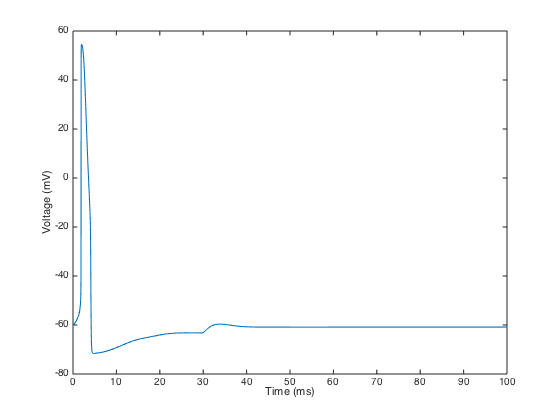
\includegraphics[scale=0.45]{motnq19.png} \caption[h17]{Anode-break spike for the simplified HH model} \end{figure}
%
% Q 20
%
\item "\emph{Never turn your back on a nonlinear differential equation}" -Eric Young \\ \\ Unforunately, the nullclines as I attemped to plot them wouldn't function properly for this question. I do, however, believe I understand approximately what would have happened and have done my best to outline that in the following question which asks for those details and explanation.
%
% Q 21
%
\item The anode-break behaviour is derived from the relationship between $m$, and $h$ gates. Since these parameters are no longer dependent on time, their behaviour and influence is reflected in the manifolds of the system. An analogy we could form is that the $h$ gates account for the stable manifold of the saddle node, while the $m$ gates account for the unstable. When a hyperpolarizing current is applied, the equilibrium points of the system shift such that the potential at equilibrium is higher than previous. The system then, when the current is removed, follows the trajectory from the former equilibrium point it was at along the unstable manifold. When the trajectory reaches this high value of $V$ and $n$, it runs into the stable manifold which brings it back towards the stable equilibrium point. The amplitude of the action potential is highly dependent on the differences in rate between $m$ and $h$ gates, and is shown on the phase plane by where the stable manifold exists.
\end{enumerate}
In summary, this project allowed me to gain valuable insight into the working of neuron models and their complexities. I have been able to wrap my head around the concepts in the class much more thoroughly than I had previously, and truly start to internalize all of the fundamental principles underlying these types of systems. Though I encountered difficulties with some parts and did not complete them to entirety, I feel as though I gained a lot from this project and am encouraged to try the final term project.
\pagebreak


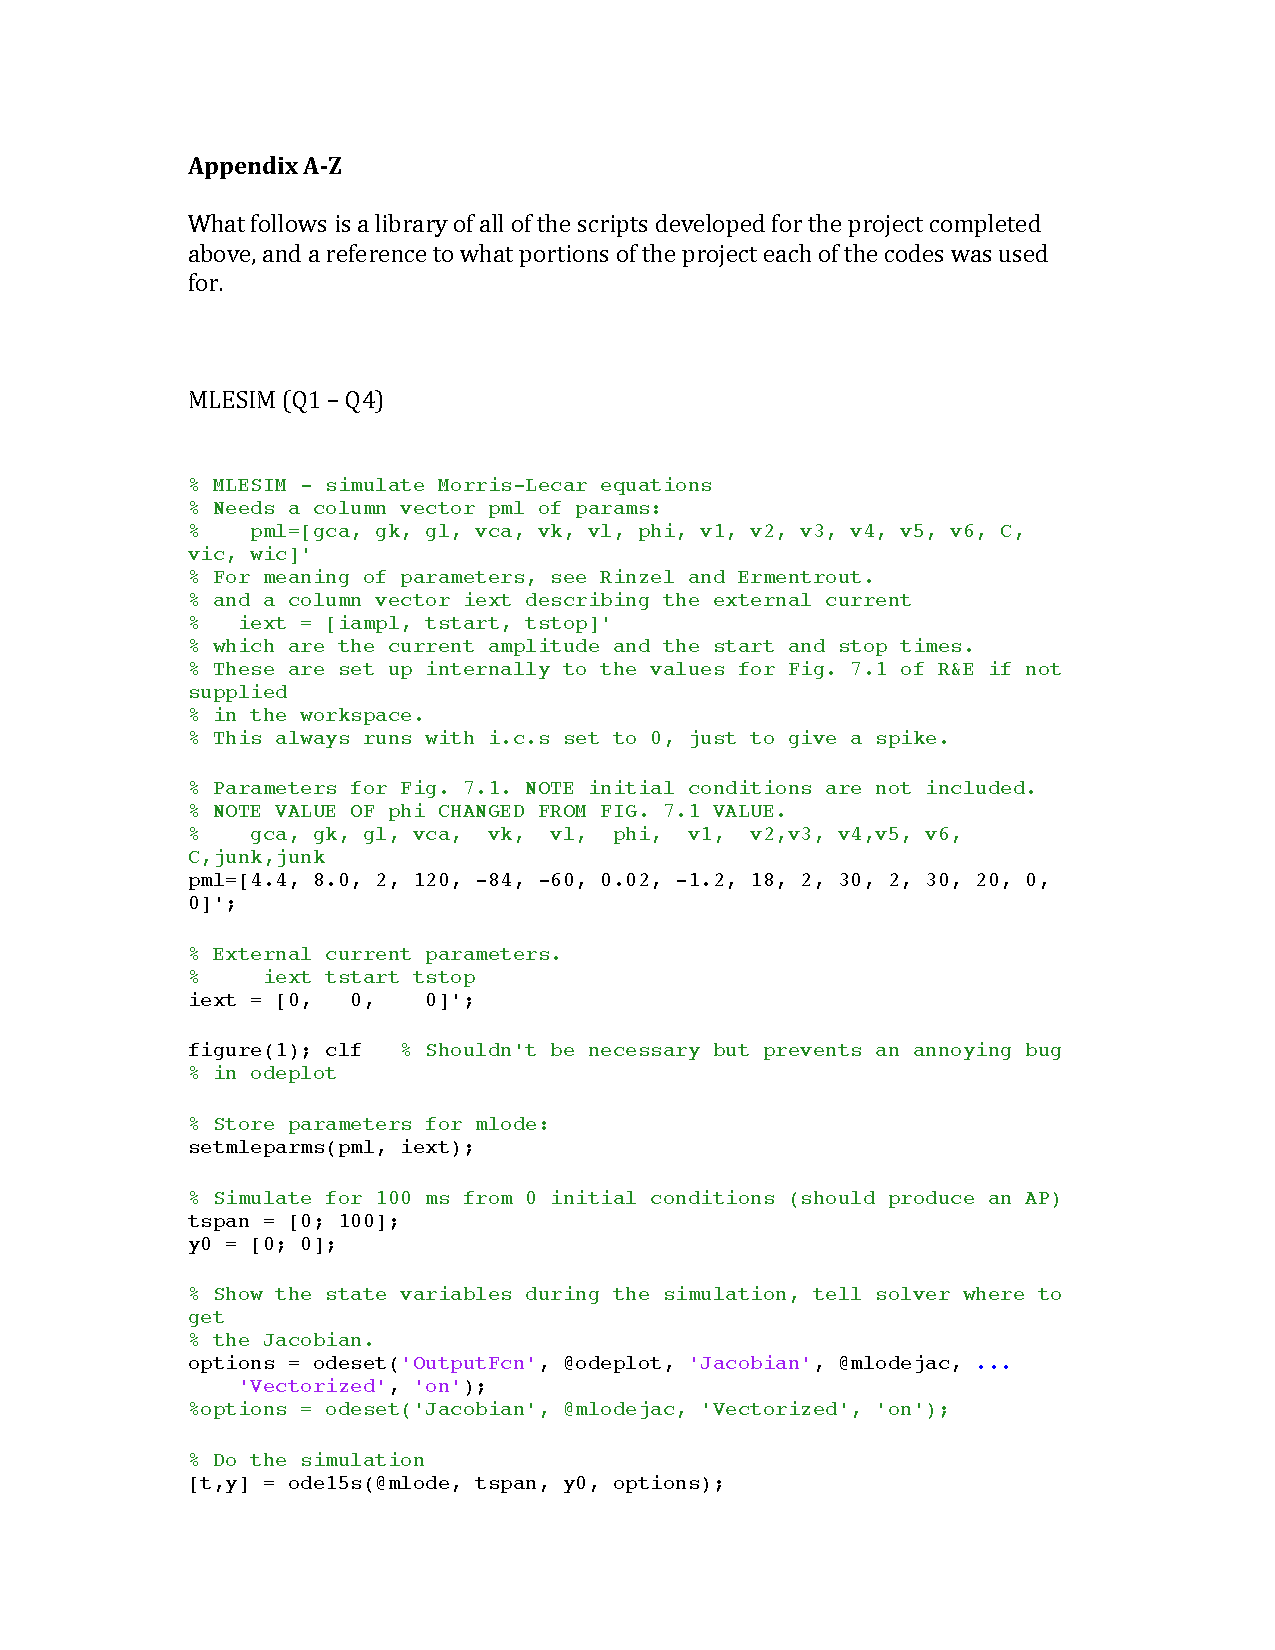
\includepdf[pages={-}]{motncode.pdf}
\end{document}
